
	\paragraph{QuizziPedia::Front-End::ModelViews::LoginModelView}
	
	\label{QuizziPedia::Front-End::ModelViews::LoginModelView}
	
	\begin{figure}[ht]
		\centering
		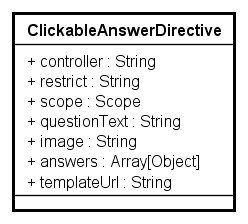
\includegraphics[scale=0.5,keepaspectratio]{UML/Classi/Front-End/QuizziPedia_Front-end_Templates_ClickableAnswerTemplate.png}
		\caption{QuizziPedia::Front-End::ModelViews::LoginModelView}
	\end{figure} \FloatBarrier
	
	\begin{itemize}
		\item \textbf{Descrizione}: ;
		\item \textbf{Utilizzo}: ;
		\item \textbf{Relazioni con altre classi}: 
		\begin{itemize}
			\item \textit{IN} \texttt{View}: ; 
			\item \textit{IN} \texttt{Controller}: ;
		\end{itemize}
		\item \textbf{Attributi}: 
		\begin{itemize}
			\item ;
		\end{itemize}
		\item \textbf{Metodi}: 
		\begin{itemize}
			\item ;
		\end{itemize}
	\end{itemize}
	
	\paragraph{QuizziPedia::Front-End::ModelViews::SignUpModelView}
	
	\label{QuizziPedia::Front-End::ModelViews::SignUpModelView}
	
	\begin{figure}[ht]
		\centering
		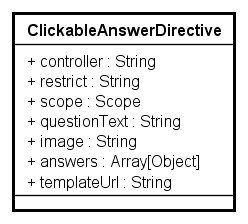
\includegraphics[scale=0.5,keepaspectratio]{UML/Classi/Front-End/QuizziPedia_Front-end_Templates_ClickableAnswerTemplate.png}
		\caption{QuizziPedia::Front-End::ModelViews::SignUpModelView}
	\end{figure} \FloatBarrier
	
	\begin{itemize}
		\item \textbf{Descrizione}: ;
		\item \textbf{Utilizzo}: ;
		\item \textbf{Relazioni con altre classi}: 
		\begin{itemize}
			\item \textit{IN} \texttt{View}: ; 
			\item \textit{IN} \texttt{Controller}: ;
		\end{itemize}
		\item \textbf{Attributi}: 
		\begin{itemize}
			\item ;
		\end{itemize}
		\item \textbf{Metodi}: 
		\begin{itemize}
			\item ;
		\end{itemize}
	\end{itemize}
	
	\paragraph{QuizziPedia::Front-End::ModelViews::PasswordForgotModelView}
	
	\label{QuizziPedia::Front-End::ModelViews::PasswordForgotModelView}
	
	\begin{figure}[ht]
		\centering
		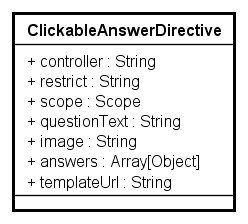
\includegraphics[scale=0.5,keepaspectratio]{UML/Classi/Front-End/QuizziPedia_Front-end_Templates_ClickableAnswerTemplate.png}
		\caption{QuizziPedia::Front-End::ModelViews::PasswordForgotModelView}
	\end{figure} \FloatBarrier
	
	\begin{itemize}
		\item \textbf{Descrizione}: ;
		\item \textbf{Utilizzo}: ;
		\item \textbf{Relazioni con altre classi}: 
		\begin{itemize}
			\item \textit{IN} \texttt{View}: ; 
			\item \textit{IN} \texttt{Controller}: ;
		\end{itemize}
		\item \textbf{Attributi}: 
		\begin{itemize}
			\item ;
		\end{itemize}
		\item \textbf{Metodi}: 
		\begin{itemize}
			\item ;
		\end{itemize}
	\end{itemize}
	
	\paragraph{QuizziPedia::Front-End::ModelViews::HomeModelView}
	
	\label{QuizziPedia::Front-End::ModelViews::HomeModelView}
	
	\begin{figure}[ht]
		\centering
		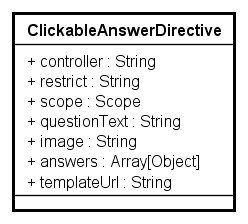
\includegraphics[scale=0.5,keepaspectratio]{UML/Classi/Front-End/QuizziPedia_Front-end_Templates_ClickableAnswerTemplate.png}
		\caption{QuizziPedia::Front-End::ModelViews::HomeModelView}
	\end{figure} \FloatBarrier
	
	\begin{itemize}
		\item \textbf{Descrizione}: ;
		\item \textbf{Utilizzo}: ;
		\item \textbf{Relazioni con altre classi}: 
		\begin{itemize}
			\item \textit{IN} \texttt{View}: ; 
			\item \textit{IN} \texttt{Controller}: ;
		\end{itemize}
		\item \textbf{Attributi}: 
		\begin{itemize}
			\item ;
		\end{itemize}
		\item \textbf{Metodi}: 
		\begin{itemize}
			\item ;
		\end{itemize}
	\end{itemize}
	
	\paragraph{QuizziPedia::Front-End::ModelViews::ResultsModelView}
	
	\label{QuizziPedia::Front-End::ModelViews::ResultsModelView}
	
	\begin{figure}[ht]
		\centering
		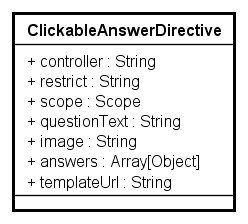
\includegraphics[scale=0.5,keepaspectratio]{UML/Classi/Front-End/QuizziPedia_Front-end_Templates_ClickableAnswerTemplate.png}
		\caption{QuizziPedia::Front-End::ModelViews::HomeModelView}
	\end{figure} \FloatBarrier
	
	\begin{itemize}
		\item \textbf{Descrizione}: ;
		\item \textbf{Utilizzo}: ;
		\item \textbf{Relazioni con altre classi}: 
		\begin{itemize}
			\item \textit{IN} \texttt{View}: ; 
			\item \textit{IN} \texttt{Controller}: ;
		\end{itemize}
		\item \textbf{Attributi}: 
		\begin{itemize}
			\item ;
		\end{itemize}
		\item \textbf{Metodi}: 
		\begin{itemize}
			\item ;
		\end{itemize}
	\end{itemize}
	
	\paragraph{QuizziPedia::Front-End::ModelViews::SearchQuestionnaireModelView}
	
	\label{QuizziPedia::Front-End::ModelViews::SearchQuestionnaireModelView}
	
	\begin{figure}[ht]
		\centering
		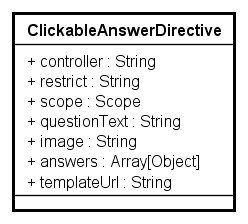
\includegraphics[scale=0.5,keepaspectratio]{UML/Classi/Front-End/QuizziPedia_Front-end_Templates_ClickableAnswerTemplate.png}
		\caption{QuizziPedia::Front-End::ModelViews::HomeModelView}
	\end{figure} \FloatBarrier
	
	\begin{itemize}
		\item \textbf{Descrizione}: ;
		\item \textbf{Utilizzo}: ;
		\item \textbf{Relazioni con altre classi}: 
		\begin{itemize}
			\item \textit{IN} \texttt{View}: ; 
			\item \textit{IN} \texttt{Controller}: ;
		\end{itemize}
		\item \textbf{Attributi}: 
		\begin{itemize}
			\item ;
		\end{itemize}
		\item \textbf{Metodi}: 
		\begin{itemize}
			\item ;
		\end{itemize}
	\end{itemize}
	
	\paragraph{QuizziPedia::Front-End::ModelViews::SearchModelModelView}
	
	\label{QuizziPedia::Front-End::ModelViews::SearchUserModelView}
	
	\begin{figure}[ht]
		\centering
		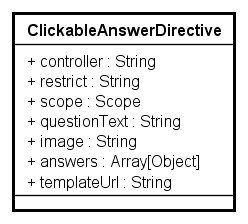
\includegraphics[scale=0.5,keepaspectratio]{UML/Classi/Front-End/QuizziPedia_Front-end_Templates_ClickableAnswerTemplate.png}
		\caption{QuizziPedia::Front-End::ModelViews::HomeModelView}
	\end{figure} \FloatBarrier
	
	\begin{itemize}
		\item \textbf{Descrizione}: ;
		\item \textbf{Utilizzo}: ;
		\item \textbf{Relazioni con altre classi}: 
		\begin{itemize}
			\item \textit{IN} \texttt{View}: ; 
			\item \textit{IN} \texttt{Controller}: ;
		\end{itemize}
		\item \textbf{Attributi}: 
		\begin{itemize}
			\item ;
		\end{itemize}
		\item \textbf{Metodi}: 
		\begin{itemize}
			\item ;
		\end{itemize}
	\end{itemize}	
